\documentclass{article}
\usepackage[utf8]{inputenc} % Permite el uso de caracteres del Español
\usepackage[T1]{fontenc}
\usepackage{hyperref}
\usepackage{graphicx}
\usepackage{wrapfig}
\usepackage{subcaption}

% Para ecuaciones
\usepackage{amssymb, amsmath, amsbsy} % simbolitos
\usepackage{upgreek} % para poner letras griegas sin cursiva
\usepackage{cancel} % para tachar
\usepackage{mathdots} % para el comando \iddots
\usepackage{mathrsfs} % para formato de letra
\usepackage{stackrel} % para el comando \stackbin

% set font encoding for PDFLaTeX or XeLaTeX
\usepackage{ifxetex}
\ifxetex
  \usepackage{fontspec}
\else
  \usepackage[T1]{fontenc}
  \usepackage[utf8]{inputenc}
  \usepackage{lmodern}
\fi

% used in maketitle
\title{Actividad 6:\\ Sistema de resortes acoplados}
\author{Melissa Matrecitos Avila}
\date{20 de Marzo de 2018}

% Enable SageTeX to run SageMath code right inside this LaTeX file.
% documentation: http://mirrors.ctan.org/macros/latex/contrib/sagetex/sagetexpackage.pdf
% \usepackage{sagetex}

\begin{document}
\maketitle
\section{Introducción}
El siguiente reporte corresponde a la actividad 6 del curso de Física Computacional 1, en la cual se enfocó en la modelación de fenómenos físicos, apoyados con Python, en especial con un sistema de resortes acoplados. Esto se logro mediante la aplicación de métodos numéricos, realizando las gráficas los resultados y comparando. cuando era posible, con la solución exacta.

Para inciar con el reporte se muestra una pequeña síntesis sobre las secciones 1 y 2 del artículo "Coupled spring equations" de  Temple H. Fay y Sarah Duncan Graham junto con las secciones de código utilizadas para resolver el problema numericamente. También se incluye la comparación de los resultados numéricos con los exactos mediante la gráfia del error relativo. Por último se presentan las secciones de conclusión, bibliografía y apéndice.

\section{Síntesis}
\subsection{Introducción}
El estudio clásico de las ecuaciones diferenciales está cambiando rápidamente, esto se debe en particular a la amplia disponibilidad de algoritmos numéricos de alta potencia y capacidades gráficas con un énfasis en las ecuaciones no lineales

En este artículo, se investiga el viejo problema de dos resortes y dos pesos unidos en serie, colgando del techo. Bajo la suposición de que las fuerzas de restauración se comportan de acuerdo con la Ley de Hooke, este problema de dos grados de libertad se modela mediante un par de ecuaciones diferenciales lineales de segundo orden acopladas. Al diferenciar y sustituir una ecuación por otra, el movimiento de cada peso se puede demostrar que está determinado por una ecuación diferencial lineal de cuarto orden.

Con las ecuaciones mencionadas se pueden estudiar algunos fenómenos más sobresalientes de este tipo de movimientos, como lo son la periodicidad, la amplitud, la fase, la sensibilidad a las condiciones iniciales y muchos otros conceptos, tan solo modificando los parámetros en el modelo.

\subsection{El modelo de resorte acoplado}
\begin{wrapfigure} {l}{0.3\textwidth}
  \centering
  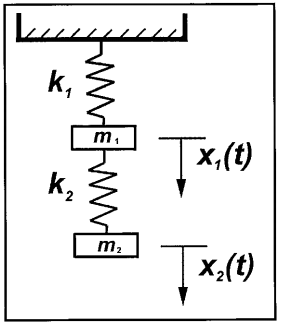
\includegraphics[width=0.25\textwidth]{SistemaResortes.PNG}
\end{wrapfigure}
El modelo consiste en dos resortes y dos pesos. Un resorte con constante $k_{1}$, está unido al techo y un peso de masa $m_{1}$ está unido al extremo inferior de este resorte. A este peso, se une un segundo resorte con una constante de resorte $k_{2}$. En la parte inferior de este segundo resorte, se adjunta un peso de masa $m_{2}$.

Considerando el sistema desde el equilibrio, medimos el desplazamiento del centro de masa de cada peso como una función del tiempo, y denotamos estas medidas por x1 (t) y x2 (t), respectivamente.

\subsubsection{Asumiendo la Ley de Hooke}
Bajo la suposición de pequeñas oscilaciones, las fuerzas de restauración son de la forma $-k_{1}l_{1}$ y $-k_{2}l_{2}$ donde $l_{1}$ y $l_{2}$ son los alargamientos (o compresiones) de los dos resortes.

Dado que la masa superior está unida a ambos resortes, hay dos fuerzas de restauración que actúan sobre ella: una fuerza de restauración hacia arriba $k1l1$ ejercida por el alargamiento (o compresión) $x1$ del primer resorte; una fuerza hacia arriba $k_{2}(x_{2}-x1)$ desde la resistencia del segundo muelle a ser alargada (o comprimida) en la cantidad $x_{2}-x1$. La segunda masa solo "siente" la fuerza de restauración desde el alargamiento (o compresión) del segundo resorte. Si asumimos que no hay fuerzas de amortiguamiento presentes, entonces la Ley de Newton implica que las dos ecuaciones que representan los movimientos de los dos pesos son:

\begin{center}
$m_{1}\ddot{x_{1}}=-k_{1}x_{1}-k_{2}(x_{1}-x_{2})$
\end{center}
\begin{center}
$m_{2}\ddot{x_{2}}=-k_{2}(x_{2}-x_{1})$
\end{center}

Para encontrar una ecuación para $x_{1}$ y $x_{2}$ que no dependan una de la otra, se resuelve la ecuación de $x_{2}$ y se sustituye en la de $x_{1}$, obteniendo las ecuaciones:
\begin{center}
$m_{1}m_{2}x_{1}^{(4)}+(m_{2}k_{1}+k_{2}(m_{1}+m_{2}))\ddot{x_{1}}+k_{1}k_{2}x_{1}=0$
$m_{1}m_{2}x_{2}^{(4)}+(m_{2}k_{1}+k_{2}(m_{1}+m_{2}))\ddot{x_{2}}+k_{1}k_{2}x_{2}=0$
\end{center}
\subsubsection{Algunos ejemplos con masas idénticas}
Considerando un sistema normalizado con masas iguales, esto es $m_{1}=m_{2}=1$, y asumiendo que no hay fricción ni fuerzas externas, la ecuación diferencial se reduce a:
\begin{center}
$m^{(4)}+(k_{1}+2k_{2})m^{2}+k_{1}k_{2}=0$
\end{center}
\textbf{Ejemplo 2.1}:\textsl{Describe el movimiento para resortes con constantes $k_{1}=6$ y $k_{2}=4$ con condiciones iniciales ($x_{1}(0),\dot{x_{1}}(0), x_{2}(0),\dot{x_{2}}(0)$)=(1,0,2,0).}

Resolviendo analíticamente encontramos que las soluciones para $x_{1}$ y $x_{2}$ son:
\begin{center}
$x_{1}(t)=\cos{\sqrt{2}t}$ \\
$x_{2}(t)=2\cos{\sqrt{2}t}$
\end{center}

El movimiento es sincronizado y las ondas se mueven fase una con la otra, teniendo el mismo periodo de movimiento pero con distintas amplitudes. Como el movimiento es periódico simple, las fases de $x_{1}$ y $x_{2}$ forman elipses.

A continuación se muestra el procedimiento correspondiente al método numérico utilizado en todos los ejemplos (variando solo las constates indicadas), este se logro utilizando Python, obteniendo los datos y guardándolos en un archivo para después ser utilizados en las gráficas como se ha hecho en prácticas pasadas:
\begin{center}
    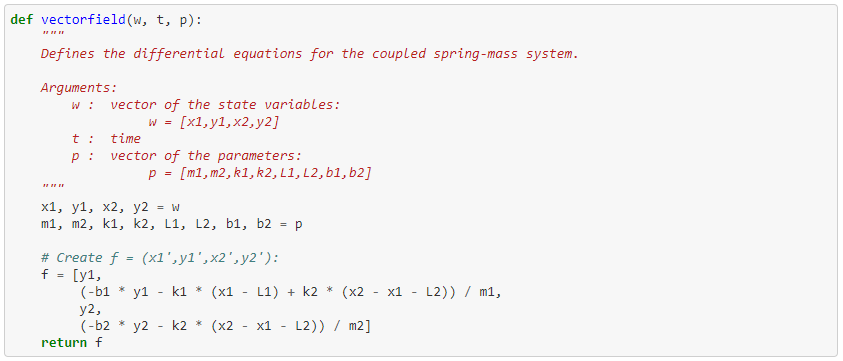
\includegraphics[width=.8\textwidth]{fun.PNG}
    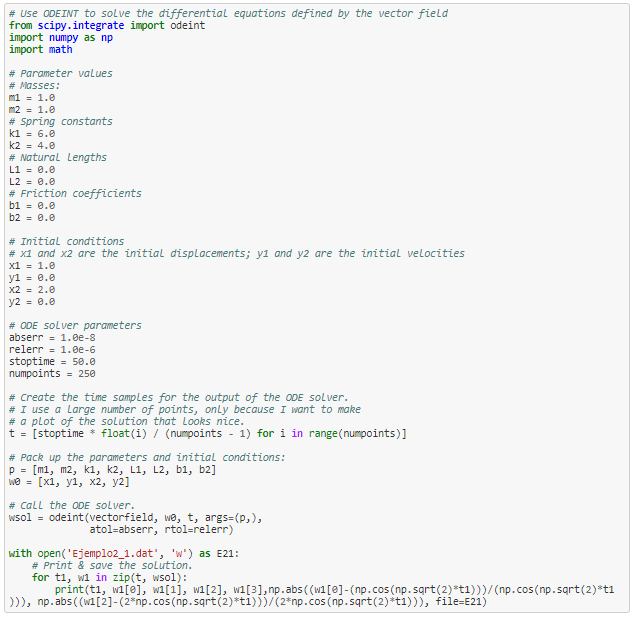
\includegraphics[width=.8\textwidth]{Datos1.PNG}
    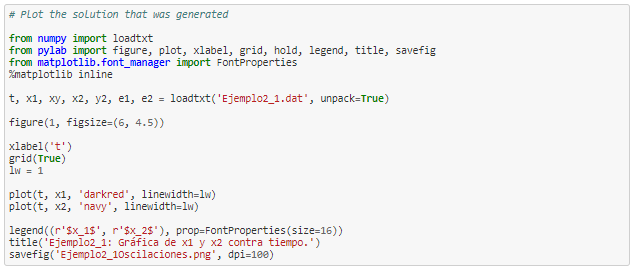
\includegraphics[width=1\textwidth]{Grafica1.PNG}
\end{center}
Las graficas obtenidas fueron:
\begin{center}
    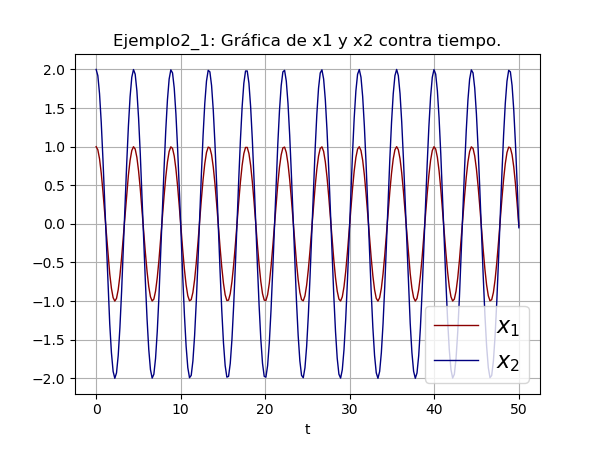
\includegraphics[width=.4\textwidth]{Ejemplo2_1Oscilaciones.png}
    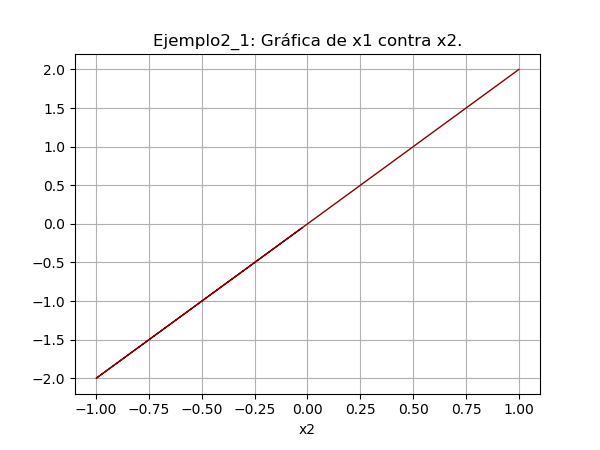
\includegraphics[width=.4\textwidth]{Ejemplo2_1Recta.png}
    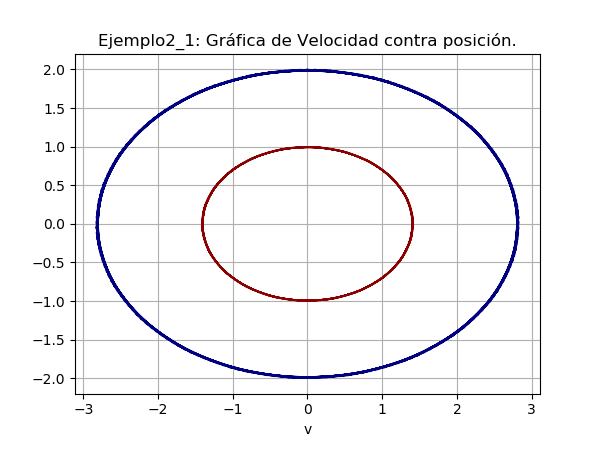
\includegraphics[width=.4\textwidth]{Ejemplo2_1Velocidad.png}
\end{center}

Cómo el articulo presenta las soluciones analíticas, es posible calcular el error relativo para la posición de cada masa, obteniendo así las gráficas del error realtivo contra el tiempo:
\begin{center}
    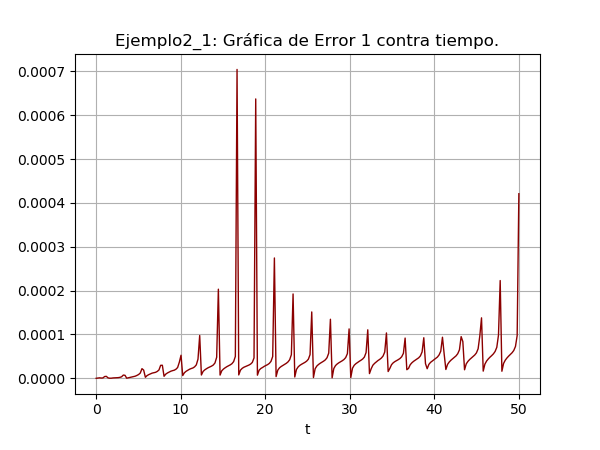
\includegraphics[width=.4\textwidth]{Ejemplo2_1Error1.png}
    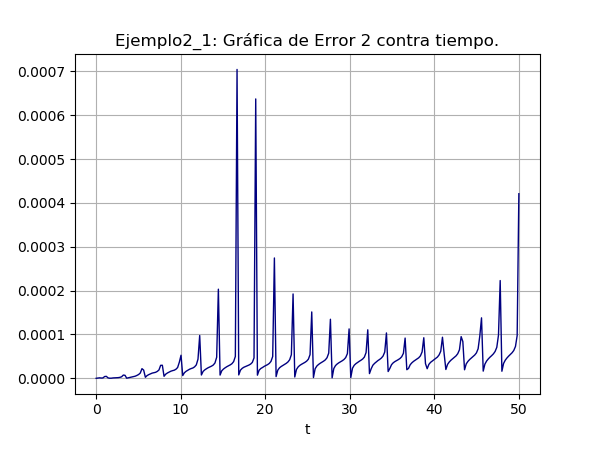
\includegraphics[width=.4\textwidth]{Ejemplo2_1Error2.png}
\end{center}

\textbf{Ejemplo 2.2}:\textsl{Describe el movimiento para resortes con constantes $k_{1}=6$ y $k_{2}=4$ con condiciones iniciales ($x_{1}(0),\dot{x_{1}}(0), x_{2}(0),\dot{x_{2}}(0)$)=(-2,0,1,0).}

Resolviendo analíticamente encontramos que las soluciones para $x_{1}$ y $x_{2}$ son:
\begin{center}
$x_{1}(t)=-2\cos{2\sqrt{3}t}$\\
$x_{2}(t)=\cos{2\sqrt{3}t}$
\end{center}
Al igual que el ejemplo anterior tienen el mismo periodo de movimiento y distintas amplitudes, solo que ahora mientras una se mueve en una dirección, la otra lo hace en sentido contrario. Así que realizando los cambios necesarios (como se muestra en la imagen) se obtuvieron las siguientes gráficas:
\begin{center}
    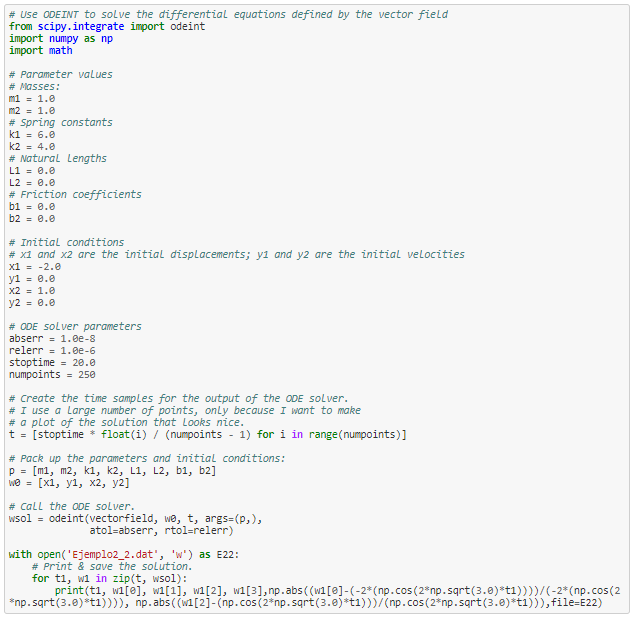
\includegraphics[width=.9\textwidth]{Datos2.PNG}
\end{center}
\begin{center}
    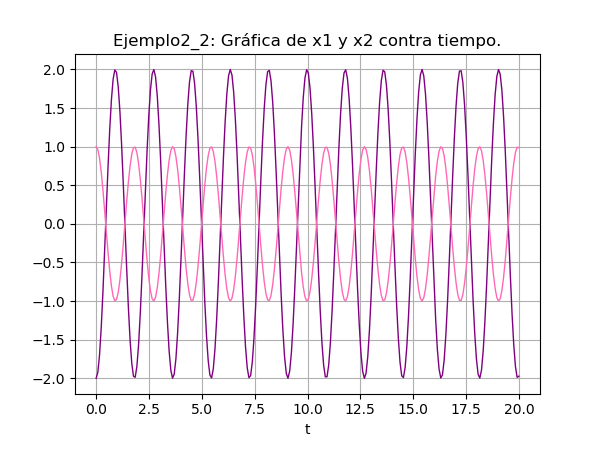
\includegraphics[width=.45\textwidth]{Ejemplo2_2Oscilaciones.png}
    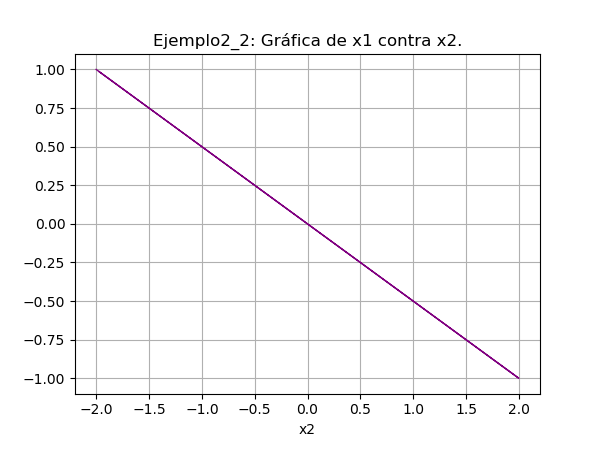
\includegraphics[width=.45\textwidth]{Ejemplo2_2Recta.png}
\end{center}

Cómo en el ejemplo anterior, el articulo también presenta las soluciones analíticas, por lo que también es posible calcular el error relativo para la posición de cada masa, obteniendo así las gráficas del error relativo contra el tiempo:
\begin{center}
    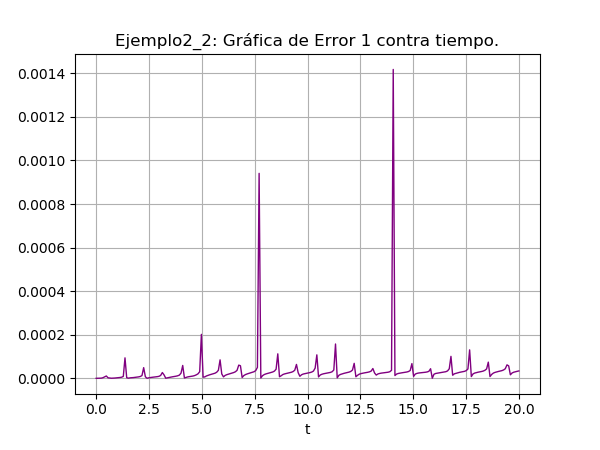
\includegraphics[width=.4\textwidth]{Ejemplo2_2Error1.png}
    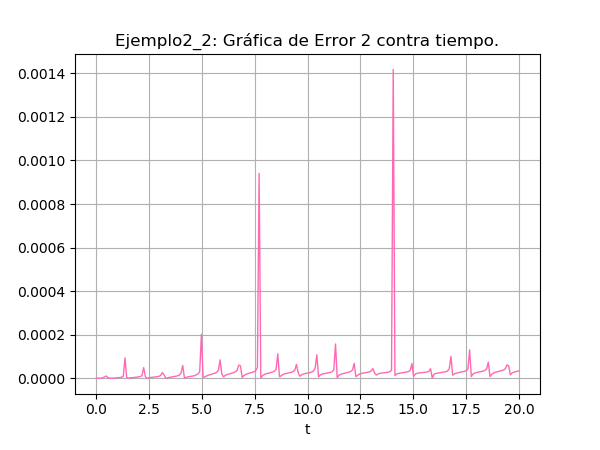
\includegraphics[width=.4\textwidth]{Ejemplo2_2Error2.png}
\end{center}

\textbf{Ejemplo 2.3}:\textsl{Describe el movimiento para resortes con constantes $k_{1}=0.4$ y $k_{2}=1.808$ con condiciones iniciales ($x_{1}(0),\dot{x_{1}}(0), x_{2}(0),\dot{x_{2}}(0)$)=(1/2,0,-1/2,7/10).}

En este ejemplo se nota como los valores de $k_{1}$ y $k_{2}$ determinan por completo el periodo y las condiciones iniciales solo afectan la amplitud y la fase de las soluciones. Este no cuenta con solución analítica, sin embargo aun se puede resolver con métodos numéricos:
\begin{center}
    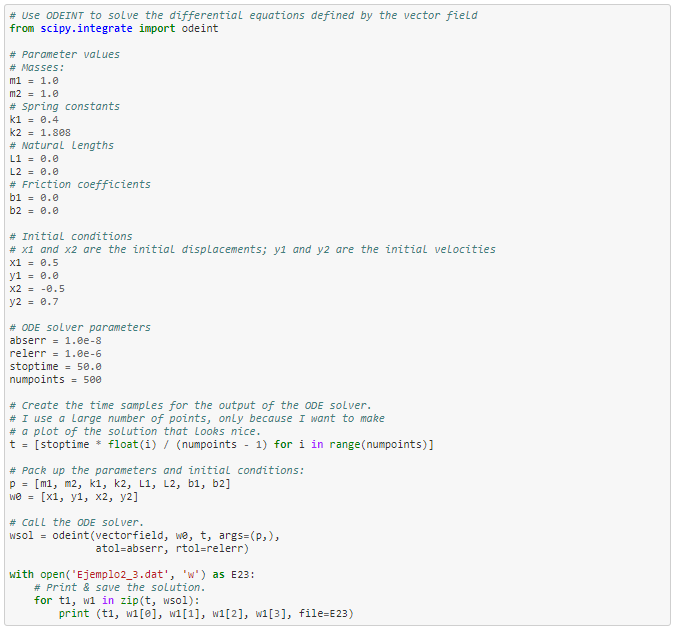
\includegraphics[width=.9\textwidth]{Datos3.PNG}
\end{center}
Obteniendo las gráficas:
\begin{center}
    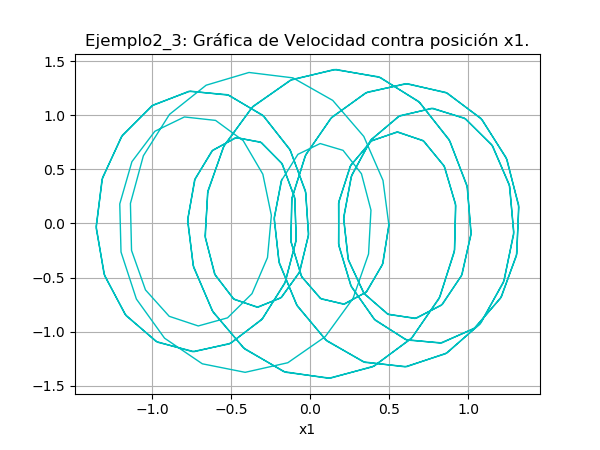
\includegraphics[width=.45\textwidth]{Ejemplo2_3Velocidad1.png}
    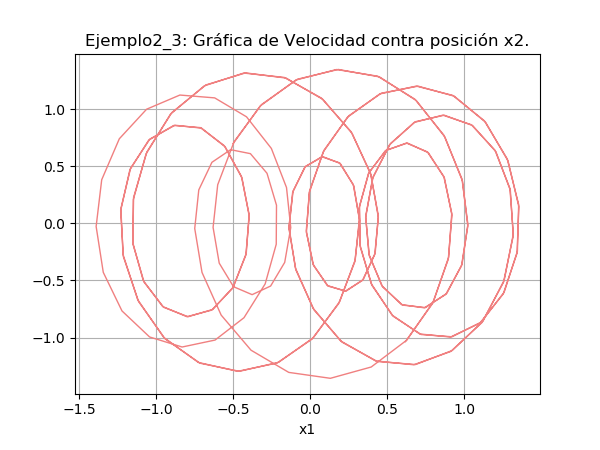
\includegraphics[width=.45\textwidth]{Ejemplo2_3Velocidad2.png}
    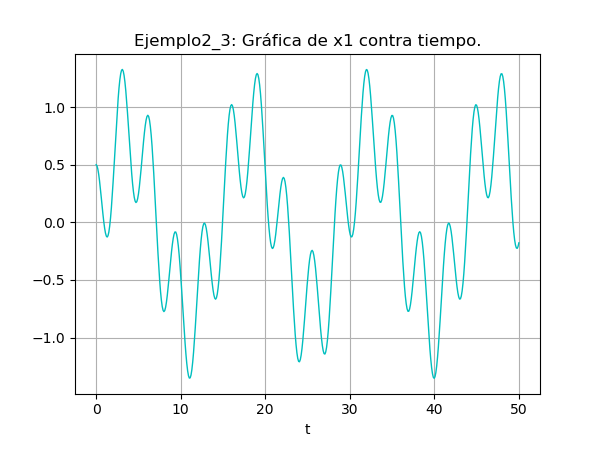
\includegraphics[width=.45\textwidth]{Ejemplo2_3Oscilaciones1.png}
    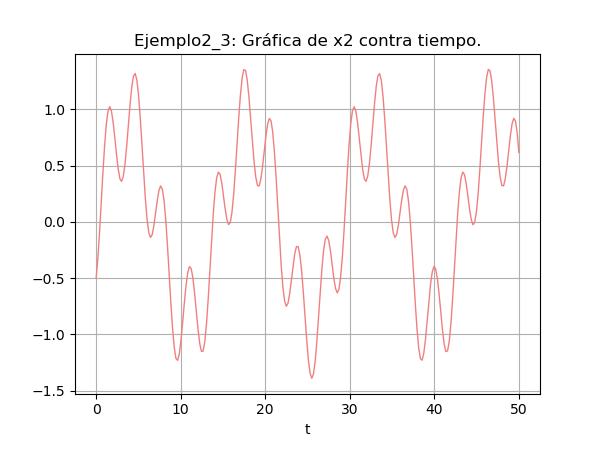
\includegraphics[width=.45\textwidth]{Ejemplo2_3Oscilaciones2.png}
    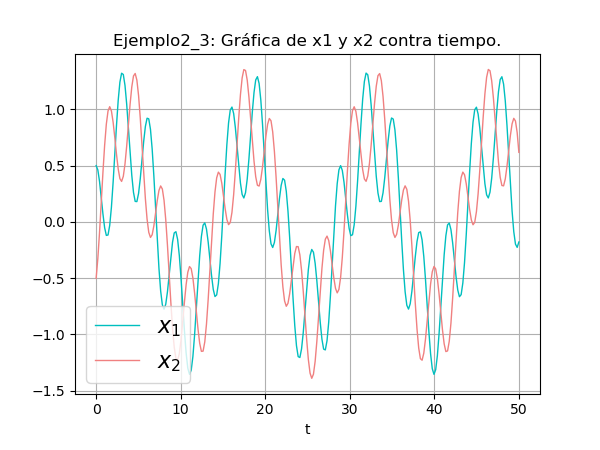
\includegraphics[width=.45\textwidth]{Ejemplo2_3Oscilaciones.png}
    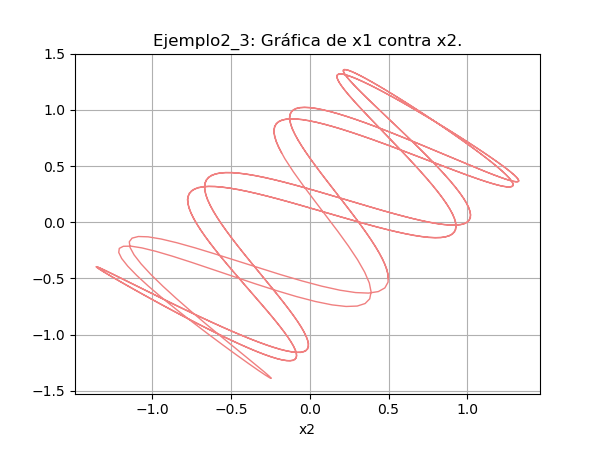
\includegraphics[width=.45\textwidth]{Ejemplo2_3Posiciones.png}
\end{center}
\subsubsection{Amortiguamiento}
EL tipo más común de amortiguamiento es el provocado por la viscosidad, donde la fuerza amortiguadora es proporcional a la velocidad. El amortiguamiento de la primera masa depende solo de su velocidad y no de la velocidad de la segunda masa y viceversa. Para agregar este fenómeno a las ecuaciones, se añaden los términos $-\delta_{1} \dot{x}_{1}$ y $-\delta_{2} \dot{x}_{2}$ a las ecuaciones correspondientes. Asumiendo que $\delta_{1}$ y $\delta_{2}$ son muy pequeños, el sistema queda:
\begin{center}
$m_{1}\ddot{x_{1}}=-\delta_{1} \dot{x}_{1}-k_{1}x_{1}-k_{2}(x_{1}-x_{2})$ \\
$m_{2}\ddot{x_{2}}=-\delta_{2} \dot{x}_{2}-k_{2}(x_{2}-x_{1})$
\end{center}
Realizando el mismo proceso para encontrar las nuevas ecuaciones para $x_{1}$ y $x_{2}$ que no dependan una de la otra, obtenemos:
\begin{center}
$m_{1}m_{2}x_{2}^{(4)}+(m_{1}\delta_{1}+m_{2}\delta_{2})\dddot{x}_{1}+(m_{2}k_{1}+k_{2}(m_{1}+m_{2}))\ddot{x_{2}}+k_{1}k_{2}x_{2}=0$
\end{center}

\textbf{Ejemplo 2.4}:\textsl{ Asuma que $m_{1}=m_{2}=1$.Describe el movimiento para resortes con constantes $k_{1}=0.4$ y $k_{2}=1.808$, coeficientes de amortiguamiento $\delta_{1}=0.1$ y $\delta_{2}=0.2$ con condiciones iniciales ($x_{1}(0),\dot{x_{1}}(0), x_{2}(0),\dot{x_{2}}(0)$)=(1,1/2,2,1/2).}


ebido al factor de amortiguamiento, la amplitud del movimiento disminuye conforme el tiempo avanza, lo cual se hace notorio en las gráficas de x1 contra tiempo y x2 contra tiempo.
\begin{center}
    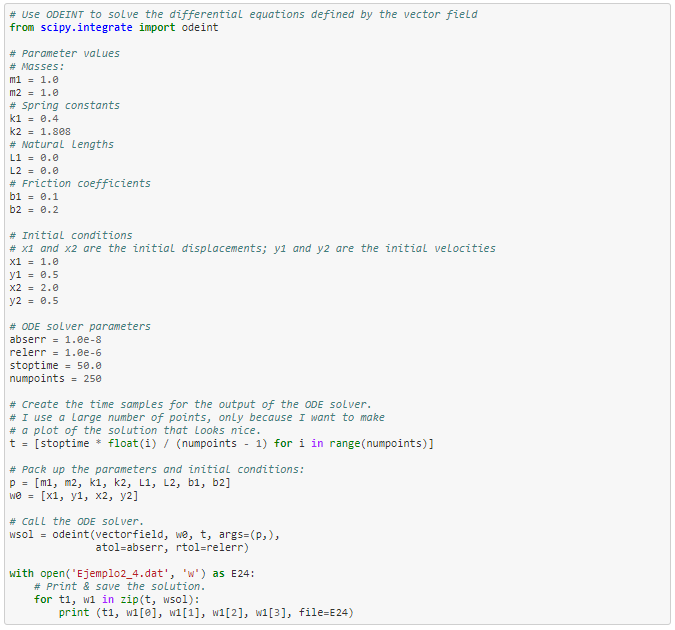
\includegraphics[width=.9\textwidth]{Datos4.PNG}
\end{center}
Obteniendo las gráficas:
\begin{center}
    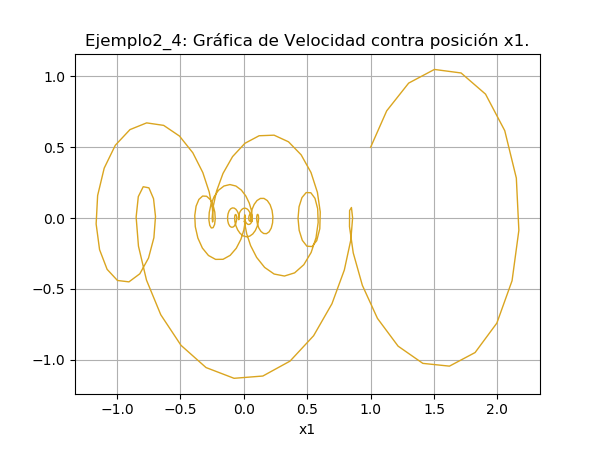
\includegraphics[width=.45\textwidth]{Ejemplo2_4Velocidad1.png}
    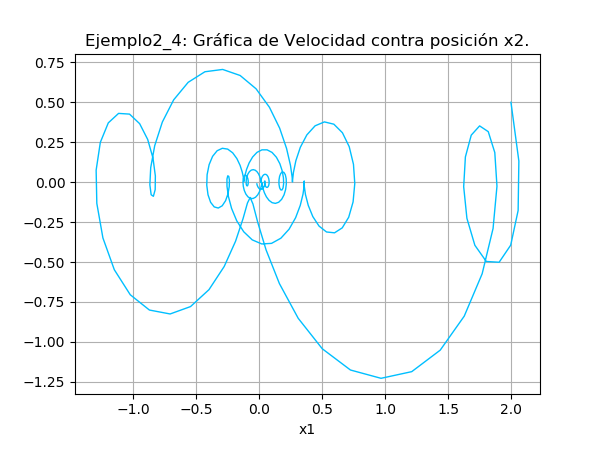
\includegraphics[width=.45\textwidth]{Ejemplo2_4Velocidad2.png}
    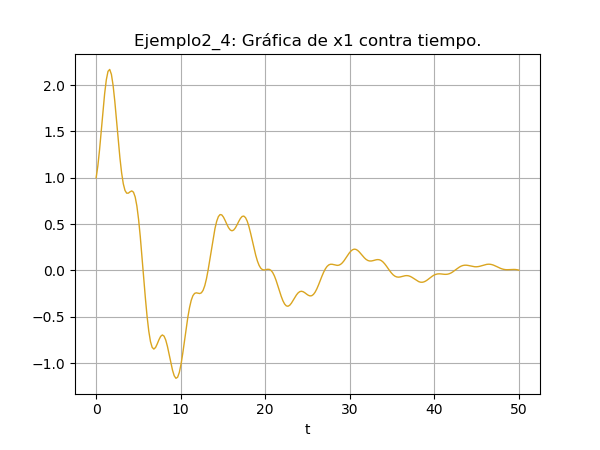
\includegraphics[width=.45\textwidth]{Ejemplo2_4Oscilaciones1.png}
    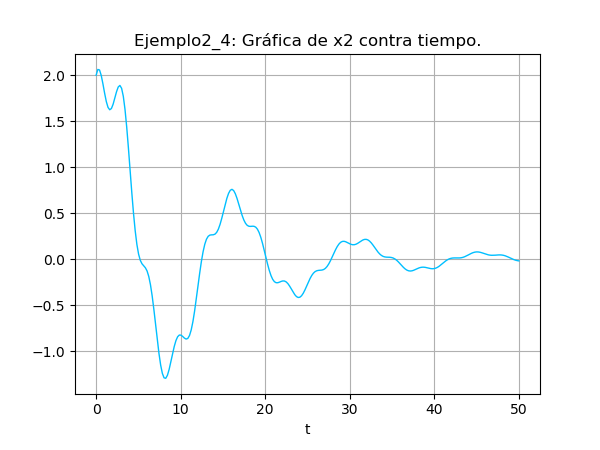
\includegraphics[width=.45\textwidth]{Ejemplo2_4Oscilaciones2.png}
    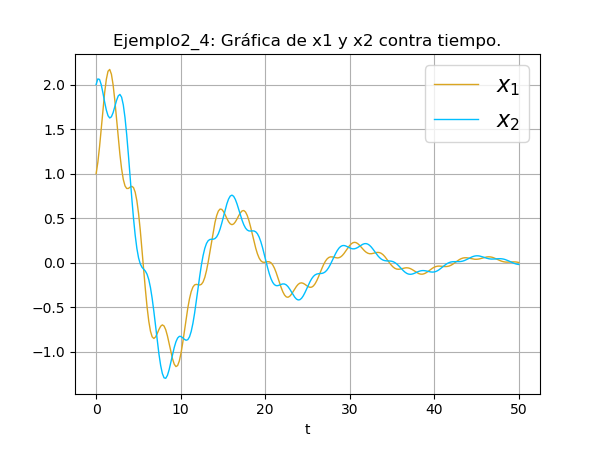
\includegraphics[width=.45\textwidth]{Ejemplo2_4Oscilaciones.png}
    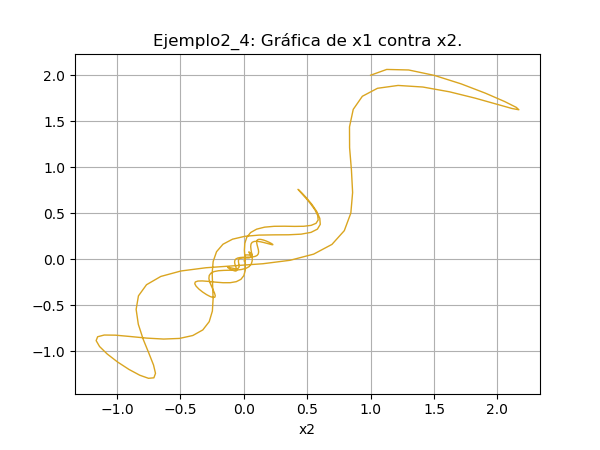
\includegraphics[width=.45\textwidth]{Ejemplo2_4Recta.png}
\end{center}

\section{Conclusión}
Trabajar con el interfaz de Jupyter Lab durante esta actividad fue de gran ayuda, ya que permite una mejor organización con los archivos, sin mencionar que las imágenes se generan inmediatamente.

Respecto al tema con el que se trabajó, se había visto en Mecánica 2, pero me pareció más sencillo visto desde la perspectiva de la programación, aun que era la primera vez que trabajaba con ecuaciones diferenciales, su solución fue muy eficaz.

\section{Bibliografía}
\begin{itemize}
\item H. FAY, T., \& DUNCAN GRAHAM, S. (2003). Coupled spring equations (pp. 65-79). Int. J. Math. Educ. Sci. Technol. Recuperado de \url{http://math.oregonstate.edu/~gibsonn/Teaching/MTH323-010S15/Supplements/coupled_spring.pdf}
\end{itemize}

\section{Apéndice}
\begin{enumerate}
\item ¿En general te pareció interesante esta actividad de modelación matemática? ¿Qué te gustó mas? ¿Qué no te gustó?

Me pareció muy interesante ya que era algo completamente nuevo para mi, aun que el código ya estaba escrito, entender como funcionaba fue muy entretenido.

\item La cantidad de material te pareció ¿bien?, ¿suficiente?, ¿demasiado?

Conforme fui realizando la actividad me pareció cada vez más adecuado.

\item ¿Cuál es tu primera impresión de Jupyter Lab?

Me pareció mucho mejor que Jupyter Notebook, debido a que era más fácil manejar los archivos y las funcioes que se pueden utilizar son más atractivas.

\item Respecto al uso de funciones de SciPy, ¿ya habías visto integración numérica en tus cursos anteriores? ¿Cuál es tu experiencia?.
Sí lo habaía visto pero era muy distinto, se habían abordado los temas de integración numérica mediante el método de trapecios y Simpson, pero no como en esta actividad, 

\item El tema de sistema de masas acopladas con resortes, ¿ya lo habías resuelto en tu curso de Mecánica 2? 
Se resolvió pero de una manera muy simple, en el curso en el que sí se aboró un poco más fue en el de Ecuaciones Diferenciales.

\item¿Qué le quitarías o agregarías a esta actividad para hacerla más interesante y divertida?
Así como está me parece muy bien.
\end{enumerate}
\end{document}
